\documentclass[hidelinks,12pt]{report}
\setcounter{tocdepth}{3} %shows all levels incl. paragraph
\usepackage[spanish]{babel}
\usepackage[tmargin=1in,bmargin=1in,lmargin=1.25in,rmargin=1.0in]{geometry}
\usepackage[T1]{fontenc}
\usepackage{graphicx}
\usepackage[usenames]{color}
\usepackage{alltt}
\usepackage{amssymb}
\usepackage{amsmath} 
\usepackage{hyperref}
\usepackage{graphicx}
\usepackage{enumitem}
\usepackage[utf8]{inputenc}
\usepackage{booktabs}
\usepackage{listings}
\usepackage{pdflscape}
\newcommand{\tabitem}{~~\llap{\textbullet}~~}
\renewcommand{\contentsname}{Índice}
\usepackage{array}
%%Jawascript definition
\usepackage{color}
\definecolor{lightgray}{rgb}{.9,.9,.9}
\definecolor{darkgray}{rgb}{.4,.4,.4}
\definecolor{purple}{rgb}{0.65, 0.12, 0.82}
\lstdefinelanguage{Javascript}{
  keywords={typeof, new, true, false, catch, function, return, null, catch, switch, var, if, in, while, do, else, case, break},
  keywordstyle=\color{blue}\bfseries,
  ndkeywords={class, export, boolean, throw, implements, import, this},
  ndkeywordstyle=\color{darkgray}\bfseries,
  identifierstyle=\color{black},
  sensitive=false,
  comment=[l]{//},
  morecomment=[s]{/*}{*/},
  commentstyle=\color{purple}\ttfamily,
  stringstyle=\color{red}\ttfamily,
  morestring=[b]',
  morestring=[b]"
}

\lstset{
   language=JavaScript,
   extendedchars=true,
   basicstyle=\footnotesize\ttfamily,
   showstringspaces=false,
   showspaces=false,
   tabsize=2,
   breaklines=true,
   captionpos=b
}

\author{[main]}
\author{Reséndiz Arteaga Juan Alberto}

\begin{document}
  %%  COVER
\pagenumbering{Alph}
\begin{titlepage}
    \begin{center}
    \begin{tabular}{r c l}
    
\includegraphics[scale=.20]{images/ipn} & \textbf{INSTITUTO POLIT\'ECNICO NACIONAL} & 
\includegraphics[scale=.20]{images/escom}\\
    & \textbf{ESCUELA SUPERIOR DE C\'OMPUTO}
    \end{tabular}
    \end{center}


    \vspace{1.5cm}
    \begin{center}


    \textbf{Computing Selected Topics:  Sistemas Complejos} \linebreak
    \large \textbf{``Juego de la Vida y Regla de Difusión''} \linebreak

    \end{center}

    \vspace{1.5cm}

    \begin{center}

    \textbf{Reséndiz Arteaga Juan Alberto} \linebreak
    \end{center}

    \vspace{1.5cm}


    %En el presente documento se encuentran los resultados correspondientes al desarrollo del Trabajo Terminal cuyo objetivo es la implementaci\'on de un sistema que analice mensajes mediante  procesamiento de lenguaje natural y teoría de reconocimiento de patrones. Este sistema pretende servir como herramienta capaz de clasificar la intención de dichas  conversaciones como peligrosas o no peligrosas. \linebreak


    \vspace{1.5cm}

    \begin{center}

    \end{center}
\end{titlepage}
\pagenumbering{arabic}

  %
\tableofcontents
\newpage
  %
\newpage
\chapter{Introducción}
  \section{Sistemas Complejos}
      \paragraph{Un sistema complejo es definido tipicamente como un sistema que es \"más que la suma de sus partes\", es decir, mientras que de forma individual los elementos del sistema pueden ser muy sencillos y fáciles de analizar, el comportamiento del sistema como un todo es altamente complejo y difícil de predecir.\cite{3}}
      \paragraph{Un sistema complejo se encuentra formado por un número elevado de componentes elementales (autómatas), que interactúan de forma local entre ellos y con el entorno que los rodea. Son sistemas cuya evolución es muy complicada de predecir ya que aparecen comportamientos (comportamiento emergente) que es difícil de predecir considerando los parámetros iniciales.}
      \paragraph{Las interacciones entre los individuos no suele ser lineal, es decir, existen proceso de retroalimentación, comunicación o inhibición en los mismos. Pueden variar su estructura con el tiempo, es decir, la creación de nuevos individuos, nuevos enlaces; como un sistema dinámico. \cite{1}}
      \paragraph{Una de las premisas más grandes es la que menciona que comportamientos simples suelen dar lugar a comportamientos macroscópicos complejos, como se pudo ver al realizar el análisis de los atractores del juego de la vida de John Conway.\cite{2}}
    \subsection{Características de los sistemas complejos}
      \paragraph{Una de las principales características de los sistemas complejos es la convivencia y relación entre los elementos con el sistema y consigo mismos, por ejemplo, un agente o automáta que tiene una visibilidad limitada de sus sitema. Un claro ejemplo es la vecindad de Moore utilizada mucho en el análisis de automatas celulares.\cite{4}}
      \paragraph{Otro factor a tomar en cuenta como principio de los sistemas complejos es que todas la unidades (automatas o elementos) son considerados como trabajos en paralelo, es decir, podrían ser vistos como computadoras independientes y cuyo procesamiento no depende uno del otro.}
      \paragraph{Los sistemas complejos como un todo muestran fenómenos emergentes, fuera de las interacciones entre las unidades simples, emerge un comportamiento complejo, patrones o inteligencia. Es bien sabido que los ejemplos existen, por ejemplo las colonias de hormigas, patrones de migración, terremotos, copos de nueve, etc.}
      \paragraph{Finalmente, se pueden identificar tres aspectos de los sistemas complejos, es importante mencionar que puede ser una diversa mezcla de éstas y no todos los sistemas complejos las tienen.}
      \paragraph{\textbf{No lineal}: Este aspecto de los sistemas complejos suele ser referido como \"el efecto mariposa\", acuñado al matemático y meteorólogo Edward Norto Lorenz, pionero en el estudio de la teoría del caos. Se le llama \"no lineal\" por qué no hay una relación donde un ligero cambio pueda ser visualizado dada una cierta función, es decir, pequeños cambios implican nuevos resultados. Los sistemas no lineales son un superconjunto de los sistemas caóticos.}
      \paragraph{\textbf{Competición y cooperación}: Una de las cosas que suelen ser visualizadas en un sistema complejo es la presencia de competición y cooperación entre los elementos. Esto puede ser visualizado durante el análisis de ciertos procesos naturales, por ejemplo, el sistema inmunológico; donde se puede ver a los glóbulos blancos (Linfocítos) distribuirse, comunicarse y cooperar para la erradicación de posibles invasores al sistema. No todod los sistemas complejos pueden mostrar ese tipo de comportamiento, por ejemplo, un análisis climatológico.}
      \paragraph{\textbf{Retroalimentación}: Los sistemas complejos suelen contener retroalimentación donde la salida de un sistema se convierte en la entrada del mismo generando resultados distintos.}



  \chapter{MicroMundo: Análisis y Desarrollo}
  \section{Análisis}
    \subsection{El ecósistema como un sistema complejo}
      Un ecosistema por si mismo es un sistema complejo. Se encuentra compuesto por organismos vivos en un hábitad determinado. Plantas y animales son componentes bióticos de un ecosistema, mientras qué el agua, aire, temperatura, luz, clima y lluvias son componentes abióticos.

      Tanto los componentes bióticos como abióticos forman relaciones entre ellos que caracterízan al ecosistema como tal brindando un balance ``temporal''. De acuerdo a sus tareas dentro del ecosistema, los componentes bióticos pueden ser divididos en:

      \begin{itemize}
        \item \textbf{Productores}: Los organismos autótrofos que producen por si mismos materia orgánica que necesitan para vivir y crecer utilizando moléculas inorgánicas como agua, dióxido de carbono y nitratos, en ésta área podemos encontrar plantas, algas y algúnas bacterias.
        \item \textbf{Consumidores}: También conocidos como organismos heterótrofos, debido a que no pueden producir su propio alimento, sin embargo, pueden alimentarse o bien alimentar también a los productores (por medio de desechos orgánicos o heces fecales).
        \item \textbf{Descomponedores}: Bien son bacterias que se dedican a descomponer la materia orgánica de los tejidos u organismos muertos y regresan las moléculas al ambiente.
      \end{itemize}

      Cada ecosistema contiene una cantidad dada de materia orgánica que incluye tanto vegetales como animales, el conjunto o peso de todos los componentes se le conoce como biomasa.\cite{6}

      La relación entre los componentes mencionados es algo fundamental en el área de biología. Los ecosistemas, y ciertamente la biosfera global son prototipos de sistemas adaptativos complejos, en donde las propiedades su sistema macroscópico, como su estructura trófica (Cadena alimentícia), diversidad y productividad, patrones y flujo de nutrientes, surge de la interacción entre los componentes y ésta retroalimenta al sistema para seguir generando las relaciones antes mencionadas.

      Indudablemente, los ecosistemas muestran regularidades en estructura y funcionalidad a través de las regiones, esto extiende los patrones de la distribución de los ecosistemas hasta las variables físicas, cómo el clima de la región y características del suelo. \cite{7}

      Los sistemas complejos han ayudado a la comprensión de la ecología en muchas áreas, por ejemplo, en las fluctuaciónes de la población de un área dada. Esto ha sido logrado debido al análisis de los individuos y el modelado de simples métricas que permiten la convivencia de éstos en un ambiente dado.

      El comportamiento emergente de un ecosistema puede ser variado. Por ejemplo, la competencia y cooperación entre especies hace que éstas se adapten mejor a ciertos obstáculos naturales; también la evolución puede ser vista como un proceso emergente de la interacción, cooperación y competencia entre las especies.

      Una forma de modelar los ecosistemas es mediante agentes basados en objetivos. La meta de los agentes basados en objetivos es diseñar modelos lo suficientemente simples tales que los datos que emergen, puedan ser entendidos y puedean generar entonces un comportamiento más fácil de analizar.

      Los algoritmos genéticos son un ejemplo; éstos fueron diseñados para capturar la esencia de la evolución y adaptación y ser lo suficientemente simples para ser matemáticamente tratables. En los algoritmos genéticos se estudia la evolución de cadenas de símbolos en lugar de intentar simular el comportamiento real de los organismos. \cite{8}
  \subsection{Simulación de un MicroMundo: Un enfóque simbólico.}
  \paragraph{La idea y motivación para la realización del estudio de ecosistemas desde el enfoque complejo surge gracias a una practica escolar de la asignatura de Inteligencia Artificial tomada en la Escuela Superior de Cómputo (ESCOM) e impartida por el Dr. Salvador Godoy Calderón.}
  \paragraph{El objetivo de la práctica escolar era diseñar la lógica necesaria para poder simular el comportamiento de tres tipos de especies en un ecosistema no variable (dado por el titular de la asignatura) y lograr que las especies pudieran permanecer sin extinguirse por más de 200 generaciones.}
  \paragraph{Las búsquedas en grafos, un motor de inferencia y una base de conocimiento eran los tres principales componentes a implementar para poder lograr el objetivo. La práctica también tenía como objetivo la visualización de los elementos mediante una interfáz dada por el titular (Diseñada en Common Lisp), donde los alumnos debian adaptarse a un contrato para simplemente hacer uso de los métodos y funciones del simulador.}
  \paragraph{El caso de estudio del MicroMundo fue analizado desde un enfóque de la inteligencia artificial, considerando búsquedas, manejo de símbolos y eurísticas para poder determinar, sin embargo, al determinar el comportamiento y orden del las acciones alteraba un posible análisis estadístico. Otro problema visto durante el desarrollo del MicroMundo desde un enfoque es que los individuos (animales) carecían de un proceso de convivencia o retroalimentación, es decir, el desarrollo fue realizado de tal forma que la información de vecinos de la misma especie fuera inexistente, cosa que no pasa dentro de un ecosistema real.}
  \paragraph{Se definían ciertas reglas para que los animales pudieran moverse, comer, beber agua y eventualmente morir. Los valores dependian de cada tipo de animal además de su diferente rango de visión. A continuación se describen las reglas y valores originales desde el enfóque artificial:}
  \begin{itemize}
  \item{Existen dos tipos de plantas\: pasto y arbustos. Crecen de forma aleatoria cada día.}
  \item{Existen tres tipos de animales\: Carnívoros, Herbívoros y Carroñeros.}
    \begin{itemize}
      \item{Los herbívoros solo pueden comer arbustos y pasto.}
      \item{Los carnívoros sóo pueden comer herbívoros.}
      \item{Los caroñeros sólo pueden comer cadáveres.}
    \end{itemize}
  \item{Todos los elementos del mapa cuentan con cierta cantidad de puntos de vida, que va cambiando dependiendo las acciones realizadas.}
  \item{Un animal sólo se puede alimentar de elementos que estén en celdas contiguas y hasta la cantidad máxima de puntos vitales del alimento seleccionado o de puntos de vida del animal.}
  \item{Los animales requieren alimento y agua para sobrevivir.}
  \item{La energía de los animales se divide en puntos de alimento y puntos de agua.}
  \item{Ambas categorías deben tener un valor superior a cero par que el animal permanezca con vida.}
  \item{Los herbívoros cuentan con una visión limitada a un vecino (Vecindad de Moore), los carnívoros tienen una visión más amplia, definida por dos vecinos y los carroñeros tiene la mayor visión con tres vecinos a su alrededor.}
  \item{Los animales pueden moverse hasta el máximo de su visibilidad descontando cierta cantidad de puntos dependiendo la distancia hacía el destino (Distancia Manhattan).}
  \item{Los cadáveres permanecen inmóviles y contaminan el área contigua, disminuyendo puntos de vida a los animales y arbustos contiguos.}
  \item{El ecosistema puede ser visto como una matríz modificada de tal forma que pueda ser vista como un toroide.}
  \item{Al ser eliminado un cadáver (consumido) estos generan pasto o arbustos de forma aleatoria en sus celdas contiguas.}
  \item{Todos los animales se reproducen asexualmente con un sólo ancestro.}
  \item{Se necesita tener más de la mitad de su energía máxima para poder reproducirce.}
  \item{Al reproducirse, el animal pierde la mitad de su energía.}
  \end{itemize}
  \paragraph{Las reglas mencionadas forman parte del documento original de la práctica del \"MicroMundo\" dada en la asignatura de Inteligencia Artificial. El documento original forma parte del anexo de este proyecto.\cite{9}}
\subsection{Adaptación de la práctica: Migrando a un enfóque complejo.}
  \paragraph{El proceso de adaptación del enfóque simbólico hacia el enfoque complejo fue relativamente sencillo, sin embargo se encontraron diversos contratiempos durante el proceso de implementación. Las reglas debieron ser cambiadas y adaptadas considerando que no existiría un proceso de búsqueda y las acciones serían ejecutadas de forma aleatoria.}
  \paragraph{Otro factor importante es que ahora los elementos debían contar con un proceso mínimo de comunicación. Se debió adaptar la lógica y agregar información de lo que cada animal podía ver, sin dar datos exactos o puntuales de lo que se encontraba a su alrededor.}
  \paragraph{Se debió considerar que cada elemento del sistema era un autómata celular, tomando en cuenta las propiedades descritas previamente, tomando como limite el rango de visión de los animales, dejando algunos de tomar una vecindad de Moore como para interacción con elementos contiguos.}
  \paragraph{Otro factor importante durante la adaptación es que los puntos de vida se vieron unificados }
  \section{Desarrollo e Implementación}
  \subsection{Descripción de la implementación}    
    Principalmente la implementación se realizó utilizando técnicas como TDD y Refactor, además de utilizar ciertos conceptos de programación orientada a objetos y programación funcional.

    Después de definir las acciones que iban a realizar los objetos que iban a interactuar con el sistema se procedió a determinar los posibles valores de entrada y salida de las mismas, concepto ampliamente usado en TDD. Las pruebas fueron pensadas tomando en cuenta los distintos elementos del ecosistema, a continuación se muestra una lista de las pruebas realizadas:

      \begin{itemize}
        \item{\textbf{AnimalsTest}}
          \begin{itemize}
            \item{Morir por falta de puntos de vida}
            \item{Beber agua considerando la fuente más cercana.}
            \item{Reproducción de un nuevo animal.}
            \item{Moverse a un nuevo lugar considerando Agua/Comida/Depredadores}
            \item{Moverse a un nuevo lugar considerando la información de algún vecino dentro del rango de visión}
            \item{Comer considerando la fuente de comida más cercana.}
          \end{itemize}
        \item{CorpseTest}
          \begin{itemize}
            \item{Decrementar la vida de los elementos cercanos al cadaver}            
            \item{Generar plantas de forma aleatoria después del tiempo de vida del cadaver.}
          \end{itemize}
        \item{NatureElements}
          \begin{itemize}
            \item{Generar un mundo dada una imagen en formato PNG y colores definidos}
            \item{Generar "n" carnívoros, herbívoros, carroñeros y cadáveres de forma uniforme en un mapa.}
            \item{Convertir una planta que carece de puntos de vida en un trozo de tierra.}
          \end{itemize}
      \end{itemize}      
    
    Todas las pruebas cuentan con un mapa de prueba generado por imagenes definidas o bien como valores de entrada del mismo desarrollador. Las pruebas pueden encontrarse dentro de la carpeta \textit{Practices/src/test/}, donde se describen con máś detalle.

    Se consideró que todos los animales contaban con el mismo comportamiento, ya que las acciones son similares en todos ellos, es por eso que se decidió usar una clase que implementa todas las acciones de forma genérica, de la cual las clases que definen a los herbívoros, carnívoros y carroñeros sobreescribieran, sólo si era necesario, los métodos y su respectiva lógica.

    Considerando el trabajo previo realizado con el juego de la vida y la regla de difusión, la adaptación de la lógica del MicroMundo fue relativamente sencilla gracias al uso de Traits (Nativos del lenguaje Groovy) e implementación de polimorfismo. La estructura (propiedades y métodos) del Trait de WorldElement se define a continuación:

    \begin{itemize}
        \item{\textbf{Propiedades}}
          \begin{itemize}
            \item{\textit{alive}: Indica el estatus del objeto, vivo o muerto.}            
            \item{\textit{life}: Indica los puntos actuales de vida del objeto en cuestión.}
            \item{\textit{sightRange}: Rango de visión (Definido por las reglas del micromundo).}
            \item{\textit{position}: Ubicación en el plano x,y.}
            \item{\textit{type}: Indica el tipo de objeto, útil para el cambio de estados.}
            \item{\textit{worldCopy}: Referencia al objeto actual del mundo, se utiliza para fines de exploración.}
            \item{\textit{nearInformation}: Dentro de un objeto de tipo llave-valor indica qué elementos puede visualizar dentro de su rango.}
            \item{\textit{canonicalName}: Nombre del objeto indicando paquete y nombre de la clase, útil para la generación dinámica de objetos con comportamientos distintos.}
            \item{\textit{operations}: Instancia del objeto operations, éste objeto define arreglos con el orden de ejecución y métodos de utilería general.}
          \end{itemize}
        \item{Métodos}
          \begin{itemize}            
            \item{\textit{decreaseLife}: Realiza el decremento de la vida dado un valor.}
            \item{\textit{increaseLife}: Realiza el aumento de la vida dado un valor.}
            \item{\textit{die}: Método que ejecuta cierta acción cuando el animal muere, se sobreescribe dependiendo el animal.}
            \item{\textit{drink}: Ejecuta la acción de beber agua considerando fuentes cercanas.}
            \item{\textit{eat}: Ejecuta la acción de comer, se sobreescribe dependiendo el animal.}
            \item{\textit{locationInformation}: Ejecuta una inspección visual del animal, actualiza el campo de nearInformation para poder consultar los datos dentro de su rango de visión.}
            \item{\textit{move}: Ejecuta la acción de moverse, es aleatoria la razón.}
            \item{\textit{moveWithInformation}: Ejecuta la acción de moverse, considerando la información que el vecino más cercano tiene, la razón es aleatoria.}
          \end{itemize}        
      \end{itemize}
    Además de llevar el control de forma dinámica de las acciones que realizarán los elementos que se encuentran dentro del mundo de prueba, también es necesario gestionar las acciones propias de éste.

    Para ello se utiliza una convención semejante, definiciendo un Trait nuevo llamado \textit{MicroWorldAutomata} donde se lleva el control de los automatas (elementos del vecindario). Cuenta con una tarea única llamada \textit{task} donde se define la lógica del recorrido de los elementos del mapa y ejecucion de las acciones pertinentes. A continuación se define la estructura de dicho Trait:

      \begin{itemize}
        \item{\textbf{Propiedades}}
            \begin{itemize}
              \item{\textit{rows}: Indica el número de filas que tiene el vecindario.}
              \item{\textit{columns}: Indica el número de columnas que tiene el vecindario.}
              \item{\textit{start}: Bandera que indica si el proceso del ejecución ha comenzado.}
              \item{\textit{operation}: Instancia del objeto operations, éste objeto define arreglos con el orden de ejecución y métodos de utilería general.}
              \item{\textit{world}: Arreglo de dos dimensiones donde se encuentran los animales y elementos del ecosistema definido.}
              \item{\textit{statistics}: Lleva el conteo de los elementos activos dentro del mapa, considera agua, plantas, carnívoros, herbívoros, carroñeros, cadáveres y tierra.}
              \item{\textit{currentElements}: Guarda la referencia de cada tipo de dato en una lista para posteriormente poder dibujarla, interactua de forma directa con la interfáz gráfica.}
            \end{itemize}
          \item{Métodos}
            \begin{itemize}            
              \item{\textit{init}: Método que se encarga de inicializar variables como rows, columns y world.}
              \item{\textit{task}: Implementación de la lógica que implica el recorrido de los elementos del vecindario y el orden de las acciones a realizar.}            
            \end{itemize}        
      \end{itemize}
    El método task es de gran utilidad debido ya que nos permite contemplar trabajo a futuro sin modificar del todo la lógica existente, bastaría con generar un objeto que haga uso de las funcionalidades del trait y definir las funciones y razonamientos necesarios.

    \begin{figure}[h!]
      \centering
        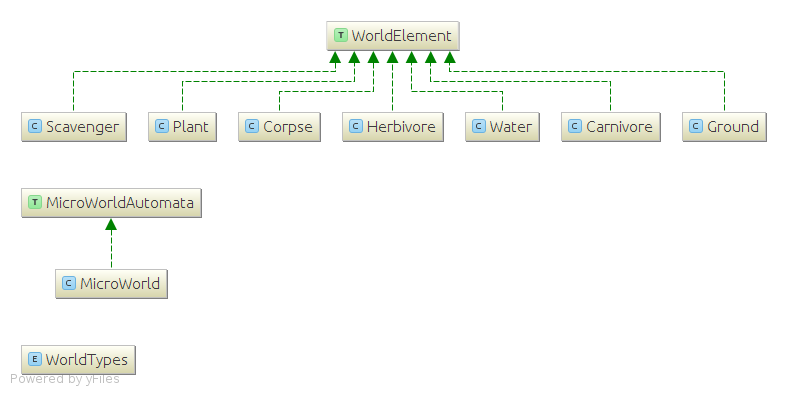
\includegraphics[scale=0.6]{./images/classDiagram}
        \caption{Diagrama de clases del MicroMundo.} 
    \end{figure}
  \newpage
  \subsection{Tecnologías}
    Se hizo uso del control de versiones Git en conjunto con su plataforma distribuida Github. Todos los códigos fuentes del proyecto pueden ser visualizados en línea a través de la siguiente liga: \url{https://github.com/jresendiz27/ComplexSystems}, dentro del mismo respositorio también se encuentran las instrucciones para poder ejecutar algun proceso, tanto del Juego de la Vida, Regla de Difusión o la simulación del MicroMundo. Las tareas que pueden ser ejecutadas fueron definidas desde Gradle.

    Gradle es otro elemento importante para el desarrollo de éste proyecto, ya que es el encargado de generar la estructura del proyecto, llevar el control de las dependencias y ejecución de tareas definidas por el usuario como; la visualización de los simuladores, el proceso de obtención de estadísticas e inserción a base de datos (Juego de la Vida y Regla de Difusión) por citar algunos.

    Se optó por realizar el trabajo usando un lenguaje multiparadigma y políglota como lo es \textbf{Groovy}. Groovy es de tipado débil y multiparadigma (Funcional y Orientado a Objetos) que se compila hacia código objeto de Java y se ejecuta sobre la JVM (Máquina Virtual de Java), es decir, cuenta con una gramática y semánticas distintas al lenguaje Java pero puede ser utilizado siguiendo las mismas normas. Esto nos trae como mayor ventaja la compatibilidad con otros sistemas que implementan o usan la JVM, además de la reutilización de bibliotecas que sólo fueron desarrolladas para Java.

    Groovy es usado durante todo el desarrollo del proyecto; debido a que la estructura del lenguaje ayuda a la generación de códigos descriptivos y menos extensos. Groovy implementa muchas operaciones con colleciones (List, Set, Map) de forma nativa sin necesidad de generar código muy extenso para poder iterar o recorrer éstas. También nos provee la ventaja de hacer uso de ciertos conceptos de programación funcional como funciones de primer orden, lambdas y closures.

    Cabe destacar que es necesario contar con Java en su versión 6 o superior para la ejecución del proyecto. Además de definir ciertos parametros en nuestras variables de entorno para que la JVM pueda gestionar mejor los recursos y poder visualizar de forma correcta los simuladores. Las variables de entorno necesarias se encuentran definidas en el archivo \textit{opts.sh} justo en la raíz del repositorio.

    El proyecto funciona siempre y cuando se le asigne un mapa (imagen llamada Sample.png, ubicada en el escritorio). Esta imagen ayudará a generar el mapa. La imágen debe tener 320 de ancho y 200 de alto; además de contener ciertos tipos de colores para las plantas, agua y tierra con los siguientes códigos hexagesimales.
      \begin{itemize}
        \item{\textit{Plantas}: 00FF00}
        \item{\textit{Tierra}: FFDEAD}
        \item{\textit{Agua}: 0000FF}
      \end{itemize}
      \begin{figure}[h!]
        \centering
          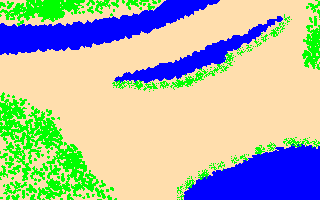
\includegraphics[width=\textwidth]{./images/Sample.png}
          \caption{Ejemplo del archivo Sample.png.} 
      \end{figure}
    Este archivo es indispensable, ya que también es usado para el proceso de generación de estadísticas. Las estadísticas se guardan en el escritorio y en un formato CSV, para que puedan ser visualizadas por Excel o de LibreOffice.
\newpage
  \subsection{Capturas de pantalla} 
    La interfáz gráfica del proyecto fue desarrollada usando Java Swing. Para el proceso de dibujado se utilizó Java2D, generando el mundo y realizando el proceso de pintado de cada elemento nuevo dentro del sistema. Por defecto el sistema carga el archivo Sample.png y lo llena con animales de forma aleatoria y uniforme tomando una distribución al 5\% del espacio libre del mundo.
    \linebreak
    \begin{figure}[h!]
      \centering
        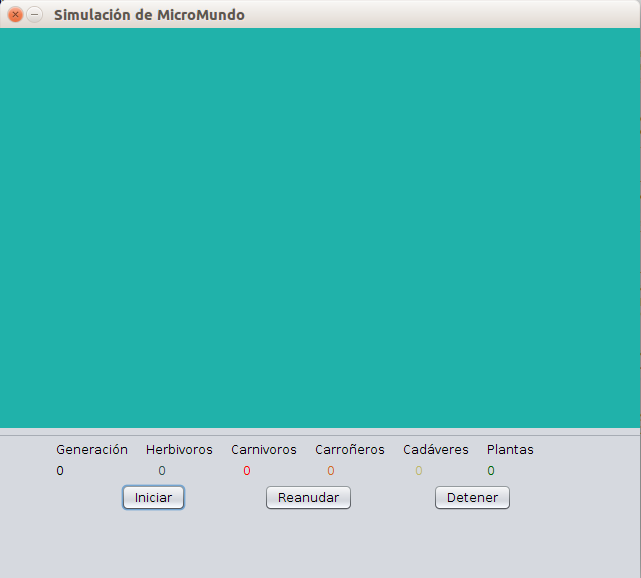
\includegraphics[scale=0.4]{./images/MicroWorldSwingInterface.png}
        \caption{Interfáz del simulador del micro mundo.} 
    \end{figure}
    \linebreak
    Los tres botones son las acciones que pueden ser realizadas durante la ejecución del simulador. Al iniciar la simulación se carga el achivo Sample.png ubicado en el escritorio y se ejecuta cada ocho segundos la lógica y dibujado del mundo. 

    Además tambien pueden verse las estadísticas actuales del mundo, tomando en cuenta la cantidad de Carnívoros, Cadáveres, Carroñeros, Herbívoros y Plantas, todo esto se obtiene por cada generación que pasa.
    \linebreak
    \begin{figure}[h!]
      \centering
        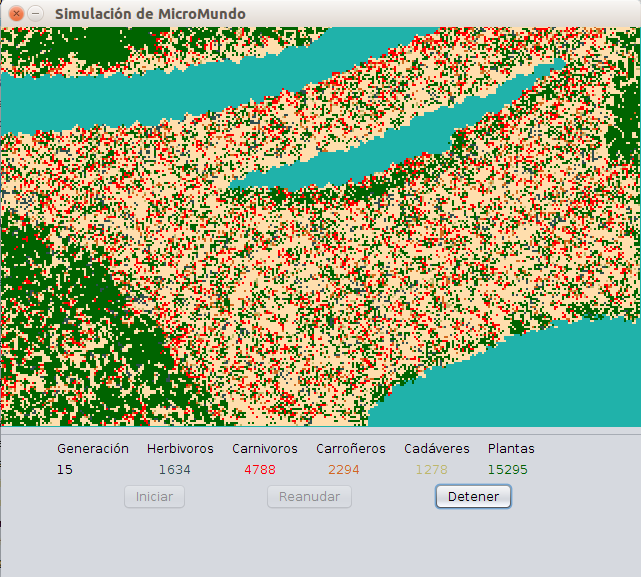
\includegraphics[scale=0.4]{./images/MicroWorldProcess.png}
        \caption{Ejecución y dibujado del MicroMundo.} 
    \end{figure}
    \linebreak
    Se tomó en cuenta el tamaño para la visualización del MicroMundo, es por ello que dentro del proceso de dibujado se escala la imágen original al doble para que pueda ser vista sin mayor problema. 

    La interfáz gráfica puede ser visualizada en ejecución desde la siguiente liga: \url{https://www.youtube.com/watch?v=AvsQTAi9elI}. 

    Se realiza una ejecución por 300 generaciones y claramente se puede visualizar el comportamiento emergente de las especies, al buscar siempre fuentes de agua y reunirse en manadas. 
  \begin{thebibliography}{1}
  \bibitem{1}
    Sistemas Complejos, Sistemas Dinámicos y Redes, Sancho Caparrini Fernando, 2011, Available at: \url{http://es.slideshare.net/FernandoCaparrini/sistemas-complejos-sistemas-dinmicos-y-redes}
  \bibitem{2}
    What is the game of life?, Paul Callahan, N/A, Available at: \url{http://www.math.com/students/wonders/life/life.html}
  \bibitem{3}
    Nature of Code, Daniel Shiffman, 2012, Availablet at: \url{http://natureofcode.com/}
  \bibitem{4}
    Moore neighborhood, Wikipedia, 2015, Available at: \url{https://en.wikipedia.org/wiki/Moore_neighborhood}
  
\end{thebibliography}

\addcontentsline{toc}{chapter}{Bibliografía}

  \newpage
\section*{Glosario}
\begin{itemize}  
  \item \textbf{Políglota}: En área informática, que tiene soporte o comprende varios lenguajes de programación.  
  \item \textbf{Simular}: Representar algo fingiendo o imitando lo qué no es.
  \item \textbf{Emular}: Imitar las acciones de otro procurando igualarlas o incluso excederlas.
  \item \textbf{Trófica}: Relacionado a la nutrición. Relativo a la cadena alimentícia.
  \item \textbf{Contrato}: Acuerdo bilateral por el cual una de las partes se obliga a desarrollar un programa de ordenador, normalmente partiendo de un programa estandar, que se ajuste a las necesidades y objetivos de la otra parte.
  \item{\textbf{Multiparadigma}: Es aquel que porta más de un paradígma de programación, por ejemplo, aquellos que implementan conceptos de programación funcional, estuctural y orientado a objetos.}
  \item{\textbf{TDD}: Test-Driven Development, técnica de desarrollo que basa su conducta en la creación de pruebas previo a la creación del código que implementará la lógica de negocio.}
  \item{\textbf{Refactor}: Técnica de desarrollo de software donde se mejora la estructura y ejecución de un trozo de código sin alteral la funcionalidad final de éste.}
  \item{\textbf{Trait}: Concepto usado en programación orientada a objetos, éste representa una colección de métodos y propiedades que pueden ser usadas para extender la funcionalidad de alguna clase.}
\end{itemize}
\addcontentsline{toc}{chapter}{Glosario}
\end{document}
